% Options for packages loaded elsewhere
% Options for packages loaded elsewhere
\PassOptionsToPackage{unicode}{hyperref}
\PassOptionsToPackage{hyphens}{url}
\PassOptionsToPackage{dvipsnames,svgnames,x11names}{xcolor}
%
\documentclass[
  english,
  11pt,
]{article}
\usepackage{xcolor}
\usepackage[margin=2.5cm]{geometry}
\usepackage{amsmath,amssymb}
\setcounter{secnumdepth}{3}
\usepackage{iftex}
\ifPDFTeX
  \usepackage[T1]{fontenc}
  \usepackage[utf8]{inputenc}
  \usepackage{textcomp} % provide euro and other symbols
\else % if luatex or xetex
  \usepackage{unicode-math} % this also loads fontspec
  \defaultfontfeatures{Scale=MatchLowercase}
  \defaultfontfeatures[\rmfamily]{Ligatures=TeX,Scale=1}
\fi
\usepackage{lmodern}
\ifPDFTeX\else
  % xetex/luatex font selection
\fi
% Use upquote if available, for straight quotes in verbatim environments
\IfFileExists{upquote.sty}{\usepackage{upquote}}{}
\IfFileExists{microtype.sty}{% use microtype if available
  \usepackage[]{microtype}
  \UseMicrotypeSet[protrusion]{basicmath} % disable protrusion for tt fonts
}{}
\makeatletter
\@ifundefined{KOMAClassName}{% if non-KOMA class
  \IfFileExists{parskip.sty}{%
    \usepackage{parskip}
  }{% else
    \setlength{\parindent}{0pt}
    \setlength{\parskip}{6pt plus 2pt minus 1pt}}
}{% if KOMA class
  \KOMAoptions{parskip=half}}
\makeatother
% Make \paragraph and \subparagraph free-standing
\makeatletter
\ifx\paragraph\undefined\else
  \let\oldparagraph\paragraph
  \renewcommand{\paragraph}{
    \@ifstar
      \xxxParagraphStar
      \xxxParagraphNoStar
  }
  \newcommand{\xxxParagraphStar}[1]{\oldparagraph*{#1}\mbox{}}
  \newcommand{\xxxParagraphNoStar}[1]{\oldparagraph{#1}\mbox{}}
\fi
\ifx\subparagraph\undefined\else
  \let\oldsubparagraph\subparagraph
  \renewcommand{\subparagraph}{
    \@ifstar
      \xxxSubParagraphStar
      \xxxSubParagraphNoStar
  }
  \newcommand{\xxxSubParagraphStar}[1]{\oldsubparagraph*{#1}\mbox{}}
  \newcommand{\xxxSubParagraphNoStar}[1]{\oldsubparagraph{#1}\mbox{}}
\fi
\makeatother


\usepackage{longtable,booktabs,array}
\newcounter{none} % for unnumbered tables
\usepackage{calc} % for calculating minipage widths
% Correct order of tables after \paragraph or \subparagraph
\usepackage{etoolbox}
\makeatletter
\patchcmd\longtable{\par}{\if@noskipsec\mbox{}\fi\par}{}{}
\makeatother
% Allow footnotes in longtable head/foot
\IfFileExists{footnotehyper.sty}{\usepackage{footnotehyper}}{\usepackage{footnote}}
\makesavenoteenv{longtable}
\usepackage{graphicx}
\makeatletter
\newsavebox\pandoc@box
\newcommand*\pandocbounded[1]{% scales image to fit in text height/width
  \sbox\pandoc@box{#1}%
  \Gscale@div\@tempa{\textheight}{\dimexpr\ht\pandoc@box+\dp\pandoc@box\relax}%
  \Gscale@div\@tempb{\linewidth}{\wd\pandoc@box}%
  \ifdim\@tempb\p@<\@tempa\p@\let\@tempa\@tempb\fi% select the smaller of both
  \ifdim\@tempa\p@<\p@\scalebox{\@tempa}{\usebox\pandoc@box}%
  \else\usebox{\pandoc@box}%
  \fi%
}
% Set default figure placement to htbp
\def\fps@figure{htbp}
\makeatother



\ifLuaTeX
\usepackage[bidi=basic,shorthands=off]{babel}
\else
\usepackage[bidi=default,shorthands=off]{babel}
\fi
\ifLuaTeX
  \usepackage{selnolig} % disable illegal ligatures
\fi


\setlength{\emergencystretch}{3em} % prevent overfull lines

\providecommand{\tightlist}{%
  \setlength{\itemsep}{0pt}\setlength{\parskip}{0pt}}



 


\renewcommand{\and}{\par}
\setlength{\headheight}{30pt}
\usepackage{graphicx}
\usepackage{xcolor}
\usepackage{float}
\usepackage{placeins}
\usepackage{longtable}
\usepackage{caption}
\usepackage{fancyhdr}
\usepackage{needspace}
\usepackage{array}
\usepackage{amsmath}
\renewcommand{\headrulewidth}{0pt}

\raggedbottom
\captionsetup[figure]{skip=2pt}
\newcommand{\legendfont}{\fontsize{10pt}{10pt}\bfseries\selectfont}
\newcommand{\resetfont}{\normalsize\normalfont}

%  Väljer språk för automatiska titlar -->

% \selectlanguage{english}

%  Byter språket på figur- och tabellbeskrivningar till angivna namn

\captionsetup[table]{name = Table}
\setcounter{table}{0}
\captionsetup[figure]{name = Figure}
\setcounter{figure}{0}

%  Anger att tabellbeskrivningar hamnar ovanför tabellen

\floatstyle{plaintop}
\restylefloat{table}

%  Anger sidnumreringens position

\fancyhf{}
\fancyfoot[C]{\thepage}
\pagestyle{fancy}

\fancyhead[L]{\itshape\footnotesize{732A99 Machine Learning - Lab Report}}
\fancyhead[R]{\itshape\footnotesize{jonda228, jonha849, kerar739}}

% lot and lof
\usepackage{etoolbox}
\pretocmd{\listoffigures}{\clearpage}{}{}
\apptocmd{\listoftables}{\clearpage}{}{}

\setcounter{secnumdepth}{3}
\setcounter{tocdepth}{3}
\setlength{\parskip}{\smallskipamount}
\setlength{\parindent}{0pt}

% \usepackage{titlesec}
% \titleformat{\chapter}
%    {\normalfont\LARGE\bfseries}{\thechapter.}{1em}{}
% \titlespacing{\chapter}{0pt}{50pt}{2\baselineskip}

\usepackage{ragged2e}

% custom command for thesis front page + 1
\newcommand{\makereportfrontpage}{
\begin{titlepage}
\clearpage\thispagestyle{empty}
\centering
\vspace{2cm}

{\large Master's Programme in Statistics and Machine Learning \par}
\vspace{4cm}
{\Huge 732A99 Machine Learning\par}
\vspace{1cm}
{\Huge Computer Lab 1 Block 1\par}
\vspace{1cm}
{\Huge Lab Report \par}


\vspace{2cm}

{\normalsize Jonas Danielsson \\ jonda228 \par}
{\normalsize Jonas Hautamäki Bengtsson \\ jonha849 \par}
{\normalsize Kerstin Arbring \\ kerar739 \par}
\vspace{3cm}

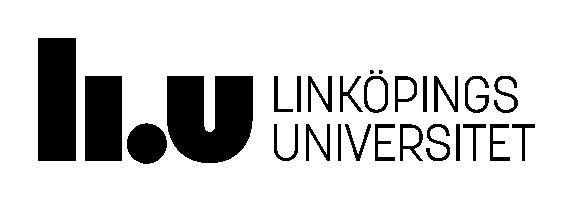
\includegraphics[scale=2]{liu_logga.png}

\vfill

{\normalsize
Division of Statistics and Machine Learning\\
Department of Computer and Information Science\\
Linköping University\\
\today\par}

\end{titlepage}

% \clearpage
% \thispagestyle{empty}
% \vspace*{\fill}
%
% \clearpage
% \setcounter{page}{1}
}
\makeatletter
\@ifpackageloaded{caption}{}{\usepackage{caption}}
\AtBeginDocument{%
\ifdefined\contentsname
  \renewcommand*\contentsname{Table of contents}
\else
  \newcommand\contentsname{Table of contents}
\fi
\ifdefined\listfigurename
  \renewcommand*\listfigurename{List of Figures}
\else
  \newcommand\listfigurename{List of Figures}
\fi
\ifdefined\listtablename
  \renewcommand*\listtablename{List of Tables}
\else
  \newcommand\listtablename{List of Tables}
\fi
\ifdefined\figurename
  \renewcommand*\figurename{Figure}
\else
  \newcommand\figurename{Figure}
\fi
\ifdefined\tablename
  \renewcommand*\tablename{Table}
\else
  \newcommand\tablename{Table}
\fi
}
\@ifpackageloaded{float}{}{\usepackage{float}}
\floatstyle{ruled}
\@ifundefined{c@chapter}{\newfloat{codelisting}{h}{lop}}{\newfloat{codelisting}{h}{lop}[chapter]}
\floatname{codelisting}{Listing}
\newcommand*\listoflistings{\listof{codelisting}{List of Listings}}
\makeatother
\makeatletter
\makeatother
\makeatletter
\@ifpackageloaded{caption}{}{\usepackage{caption}}
\@ifpackageloaded{subcaption}{}{\usepackage{subcaption}}
\makeatother
\usepackage{bookmark}
\IfFileExists{xurl.sty}{\usepackage{xurl}}{} % add URL line breaks if available
\urlstyle{same}
% fallback for those not using the hyperref driver hyperxmp:
\makeatletter
\@ifundefined{xmpquote}{\newcommand{\xmpquote}[1]{#1}}{}
\makeatother
\hypersetup{
  pdflang={en},
  colorlinks=true,
  linkcolor={blue},
  filecolor={Maroon},
  citecolor={Blue},
  urlcolor={Blue},
  pdfcreator={LaTeX via pandoc}}


\author{}
\date{}
\begin{document}


\section{Assignment 2 - Linear regression and ridge
regression}\label{assignment-2---linear-regression-and-ridge-regression}

\subsection{Data and ordinary linear
regression}\label{data-and-ordinary-linear-regression}

We predicted motor UPDRS from 16 voice characteristics in the
Parkinson's dataset. The data were randomly divided into 3525 training
observations (60\%) and 2350 test observations (40\%), using
\texttt{set.seed(12345)}. Both the predictors and response were
standardized using the \emph{training-set} means and standard
deviations, and the same transformation was applied to the test set.
Consequently, the models were fitted without an intercept.

The ordinary least squares (OLS) model had training MSE 0.8785 and test
MSE 0.9354 (on the standardized response scale). 8 coefficients were
significant at the 5\% level: Jitter(Abs), Shimmer, Shimmer:APQ5,
Shimmer:APQ11, NHR, HNR, DFA, PPE. These tests concern each coefficient
conditional on the other predictors.

\subsection{Likelihood, Ridge objective and degrees of
freedom}\label{likelihood-ridge-objective-and-degrees-of-freedom}

We assumed independent Gaussian errors, with conditional response
distribution and log-likelihood

\[
Y_i\mid \mathbf{x}_i \sim N(\mathbf{x}_i^\top\boldsymbol\theta,\sigma^2),
\qquad
\ell(\boldsymbol\theta,\sigma)
=-\frac{n}{2}\log(2\pi\sigma^2)
-\frac{1}{2\sigma^2}\sum_{i=1}^{n}
(y_i-\mathbf{x}_i^\top\boldsymbol\theta)^2.
\]

The implemented \texttt{Ridge} function evaluates the negative
log-likelihood with an L2 penalty:

\[
J(\boldsymbol\theta,\sigma;\lambda)
=-\ell(\boldsymbol\theta,\sigma)
+\lambda\sum_{j=1}^{16}\theta_j^2.
\]

For each fixed \(\lambda\), \texttt{RidgeOpt} minimizes this objective
using \texttt{optim(method\ =\ "BFGS")}, jointly estimating the
coefficients and \(\sigma\). We optimized \(\log\sigma\) instead of
\(\sigma\) directly to enforce \(\sigma>0\).

Following Lecture 1d (slides 17 and 22), the \texttt{DF} function uses
the trace of the Ridge smoother matrix to measure effective model
complexity:

\[
\operatorname{df}(\lambda)
=\operatorname{tr}\!\left[
X(X^\top X+\lambda I)^{-1}X^\top
\right].
\]

\subsection{Comparison of penalty
strengths}\label{comparison-of-penalty-strengths}

The fitted coefficients were used to predict responses by
\(\hat{\mathbf y}=X\hat{\boldsymbol\theta}\). Table
Table~\ref{tbl-a2-models} compares the training and test MSE and the
effective degrees of freedom for the three specified penalty strengths.
The estimated error standard deviation is included for completeness.

\begin{longtable}[]{@{}lrrrr@{}}

\caption{\label{tbl-a2-models}OLS and Ridge results; MSE values are on
the standardized response scale.}

\tabularnewline

\toprule\noalign{}
Model & Training MSE & Test MSE & Effective df & Sigma \\
\midrule\noalign{}
\endhead
\bottomrule\noalign{}
\endlastfoot
OLS & 0.8785 & 0.9354 & 16.0000 & 0.9373 \\
Ridge (lambda = 1) & 0.8786 & 0.9350 & 13.8607 & 0.9374 \\
Ridge (lambda = 100) & 0.8844 & 0.9323 & 9.9249 & 0.9404 \\
Ridge (lambda = 1000) & 0.9211 & 0.9540 & 5.6439 & 0.9598 \\

\end{longtable}

Among the specified penalties, \(\lambda = 100\) produced the lowest
test MSE (0.9323), compared with 0.9354 for OLS. The lecture-defined
effective degrees of freedom decreased from 13.86 at \(\lambda=1\) to
5.64 at \(\lambda=1000\). Thus, stronger regularization reduced the
model's effective flexibility, although all 16 coefficients remained in
the model. The test MSE indicates which of these penalty strengths gave
the best predictive performance on the held-out data.




\end{document}
